%
%
%
\documentclass[10pt,a4paper,oneside]{book}


%Basic stuff... more to come :)

%
%
%\documentclass[10pt,a4paper,oneside]{book}

\usepackage[slovene]{babel}
\usepackage[utf8x]{inputenc}

\usepackage{ifpdf}
\ifpdf
	\usepackage{graphicx}
	\usepackage{epstopdf}
	\epstopdfsetup{
		outdir={./img/}
	}
	\epstopdfsetup{suffix=}
	\DeclareGraphicsRule{.eps}{pdf}{.pdf}{`epstopdf --gsopt=-dEPSCrop #1}
\else
	\usepackage{graphicx}
\fi
\graphicspath{{./img/}}
\DeclareGraphicsExtensions{.eps,.pdf,.png,.jpg}

%prevent chapter pagebreaks
\usepackage{etoolbox}
\makeatletter
\patchcmd{\chapter}{\if@openright\cleardoublepage\else\clearpage\fi}{}{}{}
\makeatother

\usepackage{amsmath}
\usepackage{amsfonts}
\usepackage{amssymb}
\usepackage{tabularx}
\usepackage{url}
\usepackage{color} 
\usepackage{verbatim}
\usepackage[margin=1in]{geometry}

\usepackage{tikz}
\usetikzlibrary{calc,automata,snakes,arrows,shapes,decorations.text,positioning,shapes.arrows,chains}
\pgfmathsetseed{1}

\usepackage{lcg}

\usepackage{listingsutf8}
\lstset{
	tabsize=4,
	basicstyle={\ttfamily \scriptsize},
	identifierstyle={\ttfamily},
	inputencoding=cp1250,
	%barvanje kode
	commentstyle={\sffamily \color[rgb]{0,0.5,0}},
	stringstyle=\color[rgb]{0.5,0,1},
	keywordstyle=\color[rgb]{0,0,1},
	classoffset=0,
	%barvanje kode
	language=Java,
	deletekeywords={true,false},
	deletekeywords={byte,short,int,long,float,double,char,boolean,void},
	classoffset=1,
	morekeywords={byte,short,int,long,float,double,char,boolean,void},
	keywordstyle=\color[rgb]{0.5,0,1},
	%iz source datotek potegnemo tisto med //@begin@ ...koda... //@end@
	rangeprefix=//@,
	rangesuffix=@,
	linerange=begin-end,
	includerangemarker=false,
	%lomljenje predolgih vrstic
	breaklines=true,
	prebreak=\raisebox{0ex}[0ex][0ex]{\ensuremath{\hookleftarrow}},
	%okvir
	frame=single,
	frameround={t}{t}{t}{t},
	xleftmargin=23pt,
	xrightmargin=4pt,
	framexleftmargin=19pt,
	framerule=0pt,
	%številčenje
	numbers=left,
	firstnumber=1
}

\newenvironment{items}{
\begin{itemize}
  \setlength{\itemsep}{1pt}
  \setlength{\parskip}{0pt}
  \setlength{\parsep}{0pt}
}{\end{itemize}}

\setcounter{tocdepth}{1}

\title{Algoritmi}
\usepackage{hyperref}
\hypersetup{
    pdftitle={Algoritmi},
    colorlinks=true,
    linkcolor=black
}
\begin{document}
%\begin{comment}
\begin{titlepage}
\begin{center}
\ \\[5cm]
{\resizebox{15cm}{!}{\Huge Algoritmi}}\\[-16pt]
%{\Huge\bf Teoretične osnove računalništva}\\[1cm]
{\ \ \ \ \ \ \ \ \ \ \ \ \ \huge \today}

%"random" tikz tagclodud here?

\vfill
\parbox{7.5cm}{
\begin{center}

\includegraphics[width=0.15\textwidth]{./by-nc-sa}\\[6pt]

This work is licensed under a Creative Commons Attribution-NonCommercial-ShareAlike 3.0 Unported License
\end{center}
}

\end{center}
\end{titlepage}
\tableofcontents
\pagebreak
%\end{comment}
\begin{comment}.
\chapter{Pregled metod resevanja}
\section{Deli in vladaj}
Pri metodi deli in vladaj problem delimo na podprobleme, dokler jih ne znamo rešiti direktno, nato pa te delne rešitve sestavimo v končno rešitev. Navadno je take algoritme najlaže implementirati rekurzivno.\\
 \\
Nekaj problemov, ki jih rešujemo s to metodo:
\begin{items}
	\item Urejanje (QuickSort, MergeSort)
	\item Iskanje v urejenem seznamu (binarno iskanje)
	\item Množenje števil (Karatsubov algoritem)
	\item Množenje matrik (Strassenov algoritem)
\end{items}

\section{Dinamično programiranje}
Dinamično programiranje je v osnovi podobno metodi deli in vladaj, saj podobno problem delimo na podprobleme in nato sestavljamo končno rešitev, s to razliko, da shranjujemo vmesne rezultate. Če so podproblemi odvisni med seboj, ali na delih celo enaki, je dinamično programiranje, v primejavi z metodo deli in vladaj hitrejše, a prostorsko zahtevnejše.\\
%
%Izraz dinamično programiranje je skoval Richard Bellman že pred računalniškim programiranjem, ko se je izraz matematično programiranje uporabljal kot sopomenka optimizaciji.\\
 \\
Nekaj problemov, ki jih rešujemo s to metodo:
\begin{items}
	\item Izračun členov Fibonaccijevega zaporedja
	\item Reševanje igre Hanojski stolpi
	\item Neomejeni problem nahrbtnika
	%\item Dedno anagramska razbitja
\end{items}

\section{Požrešna metoda}
%\url{http://en.wikipedia.org/wiki/Algorithm#By_design_paradigm}
Pri požrešni metodi se, kadar imamo na voljo večih vej, odločimo za lokalno najboljšo in pri tem ne hranimo prejšnjih odločitev, ter se ne vračamo nazaj.\\
 \\
 \\
Nekaj problemov, ki jih rešujemo s to metodo:\\
%Pri NP-polnih problemih s požrešnimi algoritmi ne dobimo vedno optimalne rešitve, se ji pa navadno zelo približamo, če uporabljamo pametne hevristike:
Pri težkih problemih s požrešnimi algoritmi v splošnem ne dobimo optimalne rešitve, se ji pa lahko približamo, če uporabljamo pametne hevristike:
\begin{items}
	\item Problem trgovskega potnika
	\item Neomejeni problem nahrbtnika
\end{items}
Obstaja pa precej problemov, kjer lokalno najbolša izbira vodi tudi do končne najboljše rešitve:
\begin{items}
	\item Preprosti problem nahrbtnika
	\item Iskanje najkrajših poti v grafu (Dijkstrov algoritem)
	\item Iskanje minimalnega vpetega drevesa (Primov in Kruskalov algoritem)
	\item Izgradnja optimalnega drevesa pri Huffmanovem kodiranju.
\end{items}

%ali si razveji in omeji zasluži svoj podnaslov... in kaj je sploh razlika.
%http://wiki.answers.com/Q/What_is_Difference_between_backtracking_and_branch_and_bound_method
\section{Sestopanje in razveji \& omeji}
Sestopanje je preiskovanje celotnega prostora rešitev in najde vse možne rešitve. S pomočjo hevristik pa lahko včasih odrežemo določene veje, če ugotovimo da tam rešitve zagotovo ni, ali pa če iščemo neko bolj točno določeno rešitev. V najslabšem primeru lahko ti metodi vseeno preiščeta celoten prostor rešitev.\\
 \\
Nekaj problemov, ki jih rešujemo s to metodo:
\begin{items}
	\item Problem trgovskega potnika
	\item Problem popolnega pokritja (npr. izdelava križanke, problem osmih dam, \dots)
	\item Problem skakačevega obhoda
\end{items}

\section{Linearno programiranje}
Linearno programiranje je nastalo že pred računalniškim programiranjem in je metoda za iskanje največje vrednosti kriterijske funkcije, glede na omejitve, podane z linearnimi neenačbami.\\
\begin{comment}
 \\
Primer:\\
%primer še ni poračunan.. možno da pride kej čudnega :)
Kmet bi, glede na omejitve svojega posestva in svoj finančni položaj, rad izvedel koliko in katera semena naj kupi od zadruge, da bo njegov prihodek po žetvi največji.\\
 \\
Zadruga mu ponuja:\\
\[\begin{array}{ccccc}
\mbox{Seme} & \mbox{Prostornina $\left[\frac{m^3}{ha}\right]$} & \mbox{Cena $\left[\frac{SIT}{ha}\right]$} & \mbox{Dobiček $\left[\frac{SIT}{ha}\right]$} \vspace{2pt} \\
\hline
\mbox{Pšenica ($x_1$)}& 0.8 & 3000 & 4000 \\
\mbox{Rž ($x_2$)} & 1.2 & 2000 & 5000 \\
\mbox{Ajda ($x_3$)} & 1.0 & 3500 & 4500 \\
\end{array}\]
 \\
Njegove omejitve pa so:
\[\begin{array}{ccc}
\mbox{Ozemlje $\left[ha\right]$} & \mbox{Silos $\left[m^3\right]$} & \mbox{Proračun $\left[SIT\right]$} \vspace{2pt} \\
\hline
10 & 5 & 20000\\
\end{array}
\]
 \\
Iz teh podatkov lahko tvorimo linearni program:\\
Pogoji nenegativnosti:
\[x_1, x_2, x_3 \geq 0\]
Pogoji izpeljani iz porabe in omejitev:
\[\begin{array}{lclclcrc}
	x_1 &+& x_2 &+& x_3 &\leq& 10 & \mbox{(Ozemlje)} \\
	x_1*0.8 &+& x_2*1.2 &+& x_3*1.0 &\leq& 5 & \mbox{(Silos)} \\
	x_1*3000 &+& x_2*2000 &+& x_3*3500 &\leq& 20000 & \mbox{(Proračun)} \\
\end{array}\]
Kriterijska funkcija:
\[max(x_1*4000 + x_2*5000 + x_3*4500) \mbox{ (Dobiček)}\]
Sedaj imamo na levi strani neenačb linearno kombinacijo porabe glede na izbrano žito, na desni kmetove omejitve, v kriterijski funkciji pa kmetov dobiček, ki ga želimo maksimizirati.
\subsection{Simpleksni algoritem}
Algoritem rešuje linearne programe tako, da se sprehaja po ogljiščih konveksne poliederske množice (KPM), ki jo tvori presek danih neenačb (v 2D je KPM konveksen poligon, v 3D polieder, \dots). Pri sprehajanju se vedno premikamo le proti boljšim rešitvam, če to v nekem ogljišču ni možno, pa smo dosegli maksimum in se algoritem ustavi.

Predpostavlja se, da začenjamo iz koordinatnega izhodišča ($\forall x_i = 0$), kadar pa izhodišče ne pripada KPM, koordinatni sistem ustrezno preslikamo (premik, vrtenje, zrcaljenje, \dots).
\efnd{comment}
%Write only what you know.. :D
%Če ne najdemo ustrezne preslikave, lahko poiščemo neko nek presek enačb, ki je ogljišče KPM (), ali pa lik razrežemo in algoritem poženemo na delčkih.

%Časovna zahtevnost algoritma je v najslabšem primeru eksponentna, v praksi pa se algoritem dobro obnese, saj se sprehaja le po ogljiščih KPM in zazna, ko prispe v maksimum kriterijske funkcije.
% \\
%%TODO: Psevdokoda/Implementacija :P
\end{comment}
\chapter{Podatkovne strukture}
\section{Dvojno-povezan seznam}
\lstinputlisting[linerange=begin-end, title={Dvojno-povezan seznam}]{./src/LinkedList.java}
\section{Binarno drevo}
\lstinputlisting[linerange=begin-end, title={Binarno drevo}]{./src/BinaryTree.java}
\section{Ulomki}
\lstinputlisting[linerange=begin-end, title={Ulomki}]{./src/Fractions.java}


\chapter{Teorija stevil}

\section{Praštevila}
\begin{comment}.
Praštevila so naravna števila, ki so deljiva le z $1$ in sama s seboj. Ostalim naravnim številom, razen $1$, pravimo sestavljena števila, saj jih je moč sestaviti kot produkt praštevil.\\
\\
Kot je dokazal že Evklid\cite{elementi}, obstaja neskončno praštevil. Uporabimo preprost dokaz z protislovjem.
Predpostavimo, da imamo množico števil, ki vsebuje vsa praštevila $P = \{2,3,5,\dots,p\}$. Če sedaj vsa praštevila zmožimo in na koncu prištejemo $1$, dobimo število, ki ga ne deli nobeno izmed teh praštevil. Ker obstajajo le praštevila in števila sestavljena iz prafaktorjev, lahko sklepamo, da je to število novo praštevilo, ki ga ni v naši začetni množici, to pa je v protislovju s predpostavko. V resnici ni nujno, da je dobljeno število praštevilo -- druga možnost je, da obstaja še kako praštevilo, ki je manjše od zmnožka vseh praštevil, ki smo jih zajeli v množici $P$.\\

\[\begin{array}{ccccc}
(2)+1 &=& 3& &\mbox{(je praštevilo)}\\
(2*3)+1 &=& 7& &\mbox{(je praštevilo)}\\
(2*3*5)+1 &=& 31& &\mbox{(je praštevilo)}\\
(2*3*5*7)+1 &=& 211& &\mbox{(je praštevilo)}\\
(2*3*5*7*11)+1 &=& 2311& &\mbox{(je praštevilo)}\\
(2*3*5*7*11*13)+1 &=& 30031 &= 59*509 &\mbox{(ni praštevilo)}\\
\dots & & \dots& & \dots \\
\end{array}\]
\subsection{Preprosti algoritem za ugotavljanje praštevilskosti} 
Algoritem preveri, ali je parameter $a$ deljiv s katerim izmed naravnih števil v intervalu $\left[2, \sqrt{a}\right]$ in če takega števila ni, zaključi, da je $a$ praštevilo. Razlog, zaradi katerega lahko praštevilskost preverimo s tem intervalom (kljub temu, da bi tudi $\frac{a}{2}$ lahko delil $a$), leži v tem, da če je parameter sestavljen, je največji možen razcep na prafaktorje $\sqrt{a}*\sqrt{a}$.
\end{comment}
\lstinputlisting[linerange=begin-end, title={Preprosti algoritem za preverjanje praštevilskosti}]{./src/isPrime.java}
\begin{comment}%dooooh
Algoritem je moč nekoliko pohitriti tako, da že pred zanko preverimo ostanek pri deljenju z $2$, nato lahko zanko začnemo s $3$ in števec v vsaki iteraciji povečamo za $2$.\\
\end{comment}
% \\
%\subsection{Miller-Rabinov test}
%\url{http://en.literateprograms.org/Miller-Rabin_primality_test_(Java)}\\
%Video na temo hitrega iskanja praštevil:\\ \url{http://videolectures.net/solomon_vuk_patp/}

%\section{Razcep na prafaktorje}
%deli s praštevili dokler gre, s 3, s 5, s 7...

\section{Največji skupni delitelj in najmanjši skupni večkratnik}
\subsection{Evklidov algoritem}
\begin{comment}.
Največji skupni delitelj (angl. greatest common divisor -- GCD), je največje naravno število, ki deli vsa dana števila.
%Produkt skupnih prafaktorjev, ali
\subsection{Evklidov algoritem}
Evklidov algoritem za izračun GCD je verjetno eden najstarejših algoritmov, ki so še vedno v uporabi. Prvi ohranjen zapis je v Evklidovih Elementih\cite{elementi}, že prej pa naj bi bil znan Pitagorejcem. \\
\\
Algoritem temelji na ugotovitvi, da se GCD ne spremeni, če od večjega števila odštejemo manjšega. Če to odštevanje ponavljamo, dokler ena izmed spremenljivk ne doseže 0, je vrednost druge spremenljivke ravno GCD. Kasneje so ugotovili, da isto velja tudi za ostanek po deljenju, le da je potrebno precej manj korakov za izračun, zato raje uporabljamo ta način.
\end{comment}
\lstinputlisting[linerange=begin-end, title={Evklidov algoritem za iskanje največjega skupnega delitelja}]{./src/GCD.java}
\subsection{Najmanjši skupni večkratnik}
\begin{comment}.
Najmanjši skupni večkratnik (angl. least common multiple (LCM)) je najmanjše naravno število, ki je večkratnik danih naravnih števil.\\
%Produkt prafaktorjev, ki nastopajo v enem ali obeh številih,ali\\
Lahko ga izračunamo iz največjega skupnega delitelja po preprosti formuli:
\end{comment}
\[ \operatorname{lcm(a,b)}={a*b \over \operatorname{gcd}(a,b)}\]
%\lstinputlisting[linerange=begin-end, title={Algoritem za iskanje najmanjšega skupnega večkratnika}]{./src/LCM.java}

\begin{comment}
\section{Eulerjeva funkcija $\varphi$}
Pove koliko naravnih števil je hkrati manjših in tujih parametru funkcije.\\
Števili sta si tuji, kadar je njun največji skupni delitelj 1.\\
Za praštevila velja:\\
	\[\varphi(p) = p-1\]
Za potence praštevil velja:\\
	\[\varphi(p^m) = p^m - p^{m-1}\]
Za tuji števili $a$ in $b$ velja:\\
	\[\varphi(a*b) = \varphi(a)*\varphi(b)\]

%Ideja za preprost algoritem: Razcep na praštevila, odštevanje 1 in množenje
\end{comment}
\section{Fibonaccijevo zaporedje}
\begin{comment}.
Fibonacci je eden izmed najbolj znanih srednjeveških matematikov, ki je, med drugim, pisal tudi o zaporedju, ki je kasneje dobilo ime po njem\cite{liberabaci}. Zaporedje je predstavil na primeru idealizirane rasti populacije zajcev:\\
Recimo, da vsak par zajcev živi dve sezoni in vsako sezono ustvari en par potomcev. Imamo neko pokrajino, kjer zajcev še ni in začnemo z enim mladim parom in nato vsako sezono preštejemo nove pare. Čez eno sezono imamo en nov par, v drugi sezoni imajo potomce prva in druga generacija, tako da imamo dva nova para, hkrati pa prva generacija odmre. Naslednjo sezono imamo tri nove pare, umre pa druga generacija. Preostali pari ustvarijo pet novih parov, umre tretja generacija\dots\\
Vidimo, da je število potomcev v resnici enako velikosti zadnjih dveh generacij.\\
\\
Prvih nekaj členov Fibonaccijevega zaporedja je tako: $0,1,1,2,3,5,8,13,21,34,55,89,144,\dots$, kar lahko zapišemo z rekurzivno enačbo:\[	F(n)=
	\left\{
		\begin{array}{ccl}
			0 &;& n=0,\\
			1 &;& n=1,\\
			F(n-1)+F(n-2) &;& n>=2.
		\end{array}
	\right. \]
\\
Kvocient členov Fibonaccijevega zaporedja konvergira proti zlatemu rezu. To je moč prikazati tudi grafično, če člene zaporedja narišemo kot kvadrate ustreznih velikosti - dobimo namreč pravokotnik, katerega razmerje stranic se z dodajanjem novih členov približuje zlatemu rezu:
%kako bi sliko bolj lepo poravnal,
%oz. kako se dela vertical align
\begin{center}
\begin{tabular}{ccc}
	\begin{tabular}[b]{c|l}
		Člena & Kvocient\\
		\hline
		$1,2$ & $2$\\
		$2,3$ & $1.5$\\
		$3,5$ & $1.66\overline{6}$\\
		$5,8$ & $1.6$\\
		$\dots$ & $\dots$\\
		$987,610$ & $1.618033\dots$\\
	\end{tabular}
	&
	\begin{tabular}[b]{l}
		Zlati rez:\\
		$\varphi = \frac{1+\sqrt{5}}{2}\approx 1.618034\dots$	
	\end{tabular}
	&
	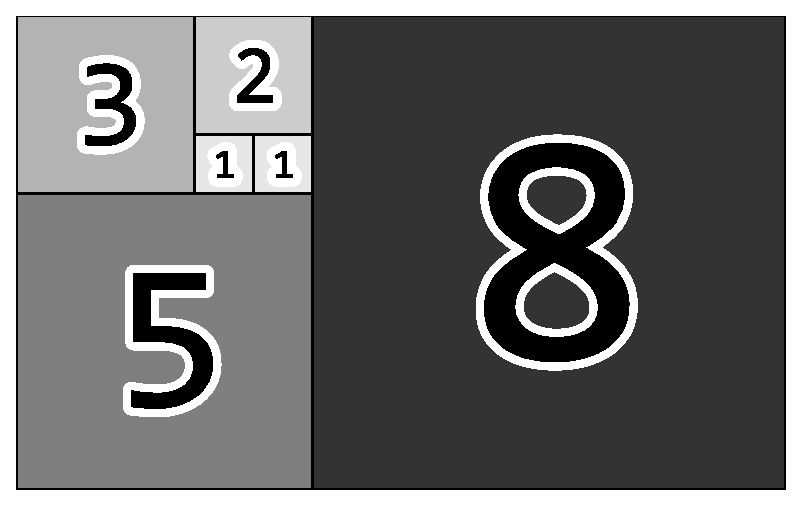
\includegraphics[width=50mm]{Fibonacci}
\end{tabular}
\end{center}
Možna posplošitev zaporedja je t.i. Fibonaccijevo zaporedje višjega reda. Če spet vzamemo Fibonaccijevo zgodbo z zajci, zaporedje višjega reda pomeni le, da zajci živijo $k$ let, namesto dveh. Pri zaporedju $k$-tega reda, torej seštejemo prejšnjih $k$ členov zaporedja.\\
 \\
Rekurzivno enačbo za Fibonaccijevo zaporedje $k$-tega reda zapišemo zapišemo kot:\\
\[	F(n)=
	\left\{
		\begin{matrix}
			0 && ; && n<k;\\
			1 && ; && n=k;\\
			F(n-1)+F(n-2)+\dots+F(n-k) &&; && n>k.
		\end{matrix}
	\right. \]
\subsection{Algoritem za izračun prvih $n$ členov Fibonaccijevega zaporedja}
Pri tem algoritmu najprej nastavimo prvih $k-1$ členov na nič in $k$-tega na ena, nato pa nove člene izračunamo kot vsoto zadnjih $k$ členov zaporedja.
\end{comment}
\lstinputlisting[linerange=begin-end, title={Algoritem za izračun prvih $n$ števil Fibonaccijevega zaporedja reda $k$}]{./src/Fib.java}

\begin{comment}.
\subsection{Algoritem za ugotavljanje pripadnosti števila Fibonaccijevemu zaporedju}
Algoritem računa člene Fibonaccijevega zaporedja $k$-tega reda in se ustavi, ko naleti na člen, ki je večji ali enak podanemu parametru. Pri računanju potrebujemo le zadnjih $k$ členov, ki pa bi jih bilo dobro hraniti tako, da nam ne bi bilo treba kakorkoli premetavati elementov tabele. Tu lahko uporabimo krožno tabelo, ki jo lahko simuliramo z navadno tabelo, če elemente naslavljamo po modulu velikosti tabele. Za izračun novega elementa bi lahko vedno znova računali vsoto vseh elementov, a to ni potrebno, saj je pri Fibonaccijevem zaporedju naslednji člen na položaju $i$ v tabeli mogoče preprosto izračunati:\\
\[\begin{array}{l}
\mbox{naslednjiClen} = 2\cdot\mbox{trenutniClen} - \mbox{tabela}[i]\\
\mbox{tabela}[i] = \mbox{trenutniClen}\\
\end{array}\]
Na primeru Fibonaccijevega zaporedja tretjega reda računamo tako:
\begin{center}
\begin{tabular}{c|c|c}
	Elementi tabele & Stara vsota & Nova vsota \\
	\hline
	$0$ $0$ $1$ & $-$ & $1$\\
	$\underline{1}$ $0$ $1$ & $1$ & $2$\\
	$1$ $\underline{2}$ $1$ & $2$ & $4$\\
	$1$ $2$ $\underline{4}$ & $4$ & $7$\\
	$\underline{7}$ $2$ $4$ & $7$ & $13$\\
	$7$ $\underline{13}$ $4$ & $13$ & $24$\\
	$7$ $13$ $\underline{24}$ & $24$ & $44$\\
\end{tabular}
\end{center}
\end{comment}
\lstinputlisting[linerange=begin-end, title={Algoritem za preverjanje, ali je število del Fibonaccijevega zaporedja reda k}]{./src/isFib.java}
\begin{comment}
\chapter{Urejanje podatkov}
Algoritmi za urejanje služijo urejanju vrstnega reda elementov v tabeli glede na neko relacijo med elementi oz. ključi elementov.
\section{Urejanje z izbiranjem (Selection Sort)}
Algoritem deluje tako, da v neurejenem delu tabele najdemo najmanjši element in ga vstavimo na konec urejenega dela tabele. Algoritem se v praksi ne uporablja zaradi počasnosti.
\lstinputlisting[linerange=begin-end, title={Algoritem za urejanje z izbiranjem}]{./src/selectionSort.java}
\section{Urejanje z zamenjevanjem (Bubble Sort)}
Algoritem začne iteracijo na začetku tabele. Najprej primerja prva dva elementa in če je prvi element večji od drugega, ju zamenja. Nato primerja drugi in tretji element in ju, če je potrebno, zamenja in tako naprej do konca tabele. Na koncu prve iteracije smo dokončno uredili zadnji element tabele, zato se lahko naslednja iteracija ustavi en element prej in vsaka naslednja iteracija še en element prej. Ko se izteče ena iteracija v kateri ne naredimo nobene zamenjave, je tabela urejena in lahko algoritem zaustavimo. Tudi ta algoritem je počasen, a njegova zahtevnosti ni vedno $O(n^2)$.
\lstinputlisting[linerange=begin-end, title={Algoritem za urejanje z zamenjevanjem}]{./src/bubbleSort.java}
\section{Urejanje z vstavljanjem (Insertion Sort)}
Algoritem doda prvi element v urejeni del tabele, nato pa se iterativno premika na naslednji neurejen element in ga v vstavi na ustrezno mesto v urejeni del. Tudi ta algoritem ima povprečno zahtevnost $O(n^2)$, je pa zaradi svoje preprostosti pri majhnem številu elementov ($< 30$) hitrejši od ostalih algoritmov, ki imajo morda manjšo časovno zahtevnost, zato ga včasih v okviru drugih algoritmov uporabimo na manjših podtabelah.
\lstinputlisting[linerange=begin-end, title={Algoritem za urejanje z vstavljanjem}]{./src/insertionSort.java}
\section{Urejanje s porazdelitvami (Quick Sort)}
%Verjetno najbolj uporabljan algoritem za urejanje. Iznašel ga je Sir C.A.R. Hoare v začetku 60'\cite{quicksort}. Je algoritem tipa deli in vladaj in deluje tako, da v dani tabeli izberemo nek element in vse elemente, ki so manjši damo na eno stran, večje pa na drugo in nato rekurzivno isto naredimo na dobljenih podtabelah. V najslabšem primeru ima tudi ta algoritem zahtevnost $O(n^2)$, v povprečju pa $O(n*log_2(n))$
\lstinputlisting[linerange=begin-end, title={Algoritem za urejanje s porazdelitvami}]{./src/quickSort.java}
\end{comment}

\chapter{Iskalni algoritmi}
\section{Binarno iskanje}
\begin{comment}.
Binarno iskanje je učinkovit algoritem za iskanje v urejeni tabeli.\\
Algoritem temelji na strategiji deli ni vladaj in sicer deluje tako, da na vsakem koraku razpolovi velikost intervala tabele, v katerem išče. To stori tako, da primerja element na sredini intervala, s ključem, ki se išče. Če je sredinski element manjši od ključa, naslednik sredinskega elementa v tabeli postane nova spodnja meja, če je sredinski element večji od ključa, pa je naslednik sredinskega elementa v tabeli nova zgornja meja. Iskanje se zaključi, ko naletimo na element, ki je enak ključu, če takega elementa v tabeli ni, pa se iskanje zaključi, ko se zgornja in spodnja meja intervala preiskovanja prekrijeta.
\end{comment}
\lstinputlisting[linerange=begin-end, title={Algoritem binarnega iskanja oz. bisekcije v urejeni tabeli}]{./src/binarySearch.java}

%todo interpolation search

\chapter{Grafi}
Graf formalno podamo kot dvojček vozlišč $V$ in povezav $E$ med vozlišči: $G=\langle V, E \rangle$.\\
Navadno uporabimo enega od naslednjih zapisov grafov:
\begin{items}
\item \textbf{Seznam sosednosti} -- za vsako vozlišče hranimo seznam povezanih vozlišč (omogoča hrambo dodatnih podatkov v vozliščih)
\item \textbf{Seznam pojavnosti} -- za vsako vozlišče hranimo seznam njegovih povezav in za vsako povezavo njen seznam vozlišč (omogoča hrambo dodatnih podatkov v vozliščih in na povezavah)
\item \textbf{Matrika sosednosti} -- kvadratna matrika vozlišč, kjer $M_{i,j} \neq 0$ pomeni povezavo med vozliščema $v_i$ in $v_j$. (omogoča hrambo ene vrednosti na povezavah)
\item \textbf{Matrika pojavnosti} -- matrika vozlišč, kjer $M_{i,j} \neq 0$ pomeni da ima vozlišče $v_i$ povezavo $e_j$. (omogoča hrambo ene vrednosti na obeh koncih povezave)
\end{items}

\section{Eulerjev in Hamiltonov graf}
\subsection{Eulerjev graf}
Graf je Eulerjev, kadar vsebuje Eulerjev cikel -- tak sprehod, ki vsako povezavo uporabi natanko enkrat in se na koncu vrne v izhodišče. \begin{comment}.
Multigraf je nadgradnja navadnih grafov s tem, da dovolimo več vzporednih povezav med dvema vozliščema in dovolimo tudi povezave vozlišč samih vase. Tudi multigraf je lahko Eulerjev. Preden poženemo algoritem lahko preverimo če graf izpolnjuje potrebne pogoje, npr. ali je povezan in ali so vsa vozlišča sode stopnje.\end{comment}

\lstinputlisting[language=GNUplot, firstnumber=0, title={Psevdokoda Fleuryjevega algoritma za iskanje Eulerjevega cikla}]{./src/Fleury.txt}
\subsection{Hamiltonov graf}
Graf je Hamiltonov, kadar vsebuje Hamiltonov cikel -- tak sprehod, ki vsako vozlišče obišče natanko enkrat in se na koncu vrne v izhodišče.

\section{Iskanje maksimalnega pretoka skozi graf}
\begin{comment}.
Predstavljamo si, da imamo nek vir tekočine, ki teče v razvejan sistem cevi, v katerem ima vsaka cev določen maksimalen pretok tekočine ($c_{i,j}$), ki ga lahko prenese med dvema točkama. Vsaka cev se steka v neko točko in iz vsake točke lahko naprej vodi več cevi. Tu seveda velja pravilo, da iz vsakega vozlišča odteka enako tekočine kot vanjo pride (tekočina se ne more nikjer zadrževati). Sistem ima poleg izvora tekočine tudi t.i ponor, kamor se tekočina na koncu izteka. Zanima nas, največ koliko tekočine lahko spravimo skozi tak sistem cevi od izvora do ponora.\\
\\
Sistem cevi predstavimo kot graf, kjer je izvor označen z prvim indeksom in ponor z zadnjim, nato pa po nekem algoritmu spreminjamo pretoke skozi cevi ($x_{i,j} \le c_{i,j}$), dokler ne najdemo maksimalnega.
\beagin{comment}
Imamo usmerjen graf z n vozlišči, radi pa bi našli maksimalen pretok od vozlišča 1 (izvor) do ponora(vozlišče n), glede na podane kapacitete povezav . Vozlišča v grafu označimo z zaporednimi številkami, kjer z 1 označimo izvor z n pa ponor,
pretok med vozliščema $i$ in $j$ pa $x_{i,j}$. Pretok je omejen s kapaciteto $0 \leq x_{i,j} \leq c_{i,j}$\\
Takoj vidimo, da je skupni pretok skozi graf $X$, navzgor omejen s kapacitetami povezav iz izvora in tudi vsot kapacitet povezav do ponora:
$0 \leq X \leq min(\sum_j {c_{1,j}}, \sum_i {c_{i,n}})$
\enad{comment}

\subsection{Ford-Fulkersonov algoritem}
Ideja algoritma je, da iščemo poti od izvora do ponora, ki še lahko sprejejo več tekočine in povečamo pretok do njih. Če take poti ni moč najti, smo našli optimalen pretok in se algoritem zaključi.\\
Pravimo, da je celotna pot je zasičena(ima največji možen pretok), če je vsaj ena povezava na njej zasičena, nezasičena pa kadar so vse povezave na njej nezasičene. Povezava je zasičena, ko po njej ne moremo povečati pretoka, torej $x_{i,j}=c_{i,j}$.\\
\\
Kadar potujemo po pozitivni (pravilno usmerjeni) povezavi, hočemo zagotoviti maksimalen pretok ($x_{i,j} = c_{i,j}$), lahko pa potujemo tudi po negativnih povezavah (obrnjenih proti toku), edina razlika je, da v tem primeru želimo minimalen pretok ($x_{i,j} = 0$).
%kako povem listingu, naj res vzame kot text? (ne kot GNUplot)
\end{comment}

\lstinputlisting[language=GNUplot, linerange=begin-end, firstnumber=0, title={Psevdokoda Ford-Fulkersonovega algoritma za iskanje maksimalnega pretoka skozi graf}]{./src/maxFlow.txt}

\section{Topološko urejanje}
\begin{comment}.
Če je usmerjen graf acikličen ga je moč urediti tako, da vozlišče z nižjo oznako vedno kaže le na vozlišča z višjimi oznakami. Tej ureditivi pravimo topološka ureditev. 
\end{comment}
\lstinputlisting[language=GNUplot, linerange=begin-end, firstnumber=0, title={Psevdokoda algoritma za topološko urejanje grafa}]{./src/topologicalSorting.txt}

\section{Iskanje najcenejših poti}
\subsection{Dijsktrov algoritem}
\begin{comment}.
Algoritem najde najcenejšo pot iz nekega začetnega vozlišča, do vseh ostalih vozlišč v grafu.
\end{comment}
\lstinputlisting[language=GNUplot, linerange=begin-end, firstnumber=0, title={Psevdokoda Dijkstovega algoritma za iskanje najcenejših poti}]{./src/Dijkstra.txt}
\begin{comment}
\subsection{Bellmanove enačbe}
Bellmanove enačbe pravijo, da je najcenejša pot od vozlišča $i$ do vozlišča $j$, vsota najcenejše poti $u_i,k$ do nekega vozlišča $k$ in cene povezave $c_{k,j}$. Kakšna pa je najcenejša pot do $k$? Spet najdemo neko vozlišče, iz katerega pridemo do $k$ prek ene povezave.\\
To izrazimo rekurzivno z Bellmanovimi enačbami:
\[	u_{i,j} =
	\left\{
		\begin{array}{cll}
			0 &;& i = j,\\
			\min \{ u_{i,k} + c_{k,j} \} &;& sicer\\
		\end{array}
	\right. \]
Vozlišča $k$ so vsa vozlišča grafa, iz katerih je mogoče priti v vozlišče $j$.
\end{comment}

\begin{comment}
\section{Preverjanje poravnanosti drevesa}
Za drevo rečemo, da je levo-poravnano, če je levo poddrevo polno, desnemu poddrevesu pa lahko manjkajo elementi le na zadnjem nivoju.
CODEDUMP :)
\lstinputlisting[linerange=begin-end, title={Algoritem za preverjanje leve poravnanosti binarnih dreves}]{./src/drevesa.java}
\end{comment}
\begin{comment}.
\chapter{Kombinatorika in verjetnost}
%%TODO: nauči se in spiši vse osnovne kombinatorične naloge :)
\section{Permutacije}
\lstinputlisting[linerange=begin-end, title={Algoritem za izračun permutacij danega niza}]{./src/Permutations.java}

\section{Metoda Monte Carlo}
Monte Carlo je verjetnostna metoda, ki deluje tako, da vzamemo neko množico v prostoru, ki je večja od dane množice katere velikost želimo oceniti, znamo pa ugotoviti, ali je neka točka znotraj te množice. Nato naključno izbiramo točke v naši množici in preverjamo ali so znotraj dane množice ali ne. Končna ocena metode je $\frac{zadetki}{poskusi}$.
\subsection{Izračun približka števila $\pi$}
V koordinatnem izhodišču narišemo krog s polmerom $1$ in kvadrat s stranico $1$ v prvem kvadrantu. Če kot zadetek štejemo točke, ki so za največ 1 oddaljene od izhodišča dobimo približek za $\frac{\pi}{4}$.

\begin{center}
	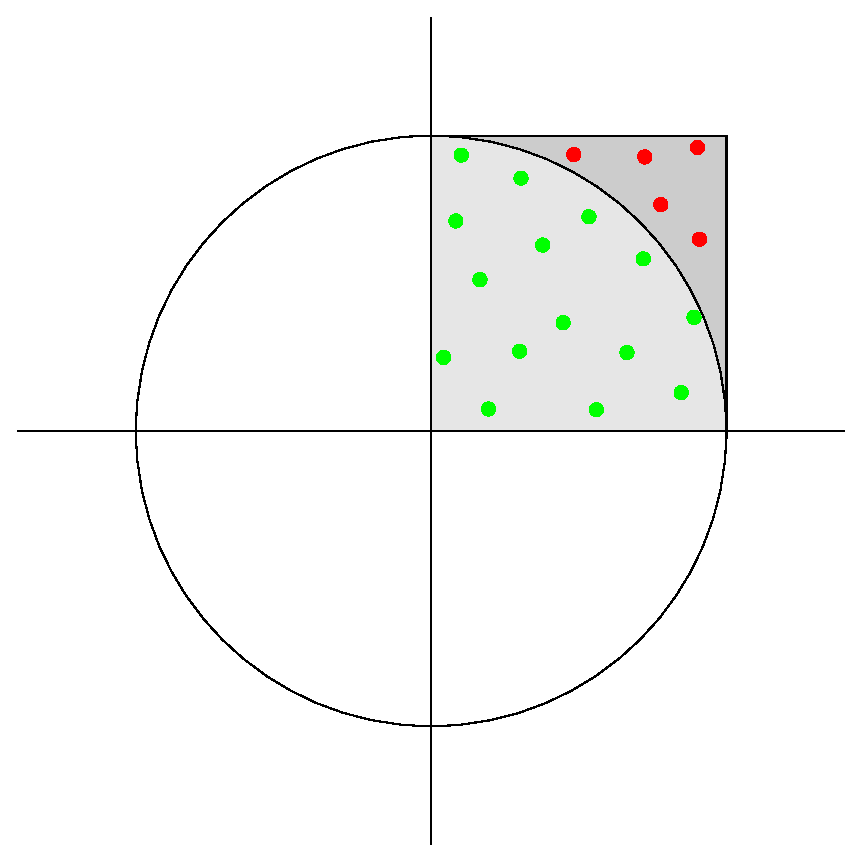
\includegraphics[width=35mm]{MonteCarloPi}
	\begidn{comment}
	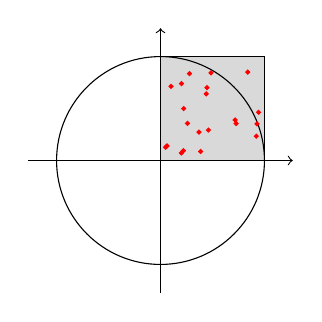
\begin{tikzpicture}[draw, scale=1.2, vertex/.style={circle,draw,fill=black,inner sep=0.5pt}]
		\draw (0, -1.4) [->] to (0, 1.4);
		\draw (-1.4, 0) [->] to (1.4, 0);
		\draw [fill=gray!30] (0, 0) rectangle (1.1,1.1);
		\draw (0, 0) circle (1.1);
		\foreach \i in {0,1,...,20} {
			\count0=1
			\count1=2
			%a^2+b^2>1 je izven kroga
			\count2=\count0
			\multiply\count2 by \count0
			\count3=\count1
			\multiply\count3 by \count1
			\count4=\count2
			\advance\count4 by \count3

			\ifnum \number\count4 > 1
				\node[vertex,draw=red,fill=red] at (rand/2 + 0.55, rand/2 + 0.55) {};
			\else 
				\node[vertex,draw=red,fill=red] at (rand,rand) {};
			\fi
		}
		%}
	\end{tikzpicture}
	\endd{comment}
\end{center}

\lstinputlisting[linerange=begin-end, title={Algoritem za izračun približka števila $\pi$ po metodi Monte Carlo}]{./src/MonteCarloPi.java}
Taka metoda za iskanje dobrega približka števila $\pi$ ni najbolj primerna, je pa preprost primer uporabe.
%Glej tudi:\\
%\url{http://www.chem.unl.edu/zeng/joy/mclab/mcintro.html}\\
%\url{www-lp.fmf.uni-lj.si/plestenjak/vaje/Nm/Gradivo/SeminarMC.pdf}
\end{comment}
\chapter{Računska geometrija}
\section{Najbližji par v množici točk}
\begin{comment}.
Želimo poiskati točki, ki sta si najbližji v neki množici točk. Naivni algoritem bi bil pregled vseh parov, kar bi zahtevalo kvadratno časovno zahtevnost, z boljšimi metodami pa dosežemo zahtevnost $O(n*log(n))$. Poglejmo preprost algoritem s pometanjem, ki ima v najboljšem primeru linearno zahtevnost, v najslabšem pa kvadratno.
\end{comment}

\lstinputlisting[linerange=begin-end, title={Preprost algoritem za iskanje najbližjega para točk v množici točk s pometanjem}]{./src/closestPair.java}
%\section{Konveksna ogrinjača množice točk}
%CODEDUMP :)
%\lstinputlisting[linerange=begin-end, title={Algoritem za iskanje konveksne ogrinjače množice točk}]{./src/convexHull.java}

%\section{Ločitev dveh množic točk s premico}
%TODO :P
%\url{http://slo-tech.com/forum/t360321#crta}

\begin{comment}
\chapter{Celularni avtomati}
\section{1D binarni avtomati}
%Program, ki generira recimo tole:\\
%\url{http://en.wikipedia.org/wiki/Rule_30}\\
Če vsaka celica gleda sebe in sosednji imamo $2^{2^3} = 256$ možnih avtomatov in tako se tudi označujejo.\\
%\url{http://en.wikipedia.org/wiki/Wolfram_code}
\section{2D binarni avtomati}
\subsection{Conwayeva igra življenja}
%\url{http://en.wikipedia.org/wiki/Conway's_Game_of_Life}
\subsection{Splošen 2D binarni avtomat}
%\url{http://en.wikipedia.org/wiki/Cellular_automaton#Overview}\\
Če vsaka celica gleda sebe in sosednjih 8 (t.i. Moorova soseska), imamo $2^{2^9}=2^{512} \approx 10^{154}$ možnih avtomatov.

\end{comment}

%\chapter{Varnostno kodiranje}
%\section{Hammingovo kodiranje}
%\lstinputlisting[linerange=begin-end, title={Algoritem za izračun Hammingovih varnostnih bitov}]{./src/Ham.java}

\chapter{Random stuff}
%\chapter{Matematične in logične igre}
\section{Možne vsote podmnožic}%from icpc
\lstinputlisting[linerange=begin-end, title={Algoritem za izračun vseh možnih vsot podmnožic neke množice}]{./src/SubsetSum.java}

\section{Hanojski stolpi}
\begin{comment}.
Hanojski stolpi je igra, ki jo sestavljajo tri palice in nekaj diskov različnih velikosti. Na začetku so diski urejeni od najmanjšega do največjega po velikosti na prvi palici, cilj igre pa je premakniti vse diske s prve palice na drugo, pri čemer ne moremo položiti večjega diska na manjšega in s palice lahko dvignemo le zgornji disk.

\begin{center}
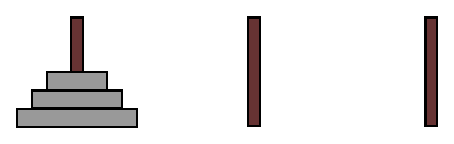
\includegraphics[width=77mm]{towersOfHanoi}
\end{center}

\subsection{Najmanjše število premikov glede na število diskov}
Če hočemo iz začetnega položaja premakniti prvi(zgornji) disk, to lahko storimo z enim premikom, če pa želimo premakniti disk pod njim, moramo najprej premakniti prvega, šele nato drugega. Po teh dveh premikih je za nadaljevanje igre potrebno eno palico sprostiti, kar dosežemo s premikom prvega diska na drugega - skupaj trije premiki. Če bi iz začetnega položaja želeli premakniti tretji disk, bi najprej s tremi premiki premaknili prva dva diska na tretjo palico, tretji disk na drugo palico, potem pa spet s tremi premiki prvi in drugi disk na drugo palico - skupaj sedem premikov. Za premik četrtega diska pa bi najprej premaknili prve tri, nato četrtega in prve tri na četrtega - petnajst premikov. Splošna formula za število premikov je: moves $= 2^n - 1$%\\
% \\
%Algoritem za izračun najmanjšega števila premikov je zelo preprost, ga je pa bolje kot z očitno rekurzijo, implementirati z uporabo dinamičnega programiranja:
%\lstinputlisting[linerange=begin-end, title={Algoritem za izračun najmanšega števila premikov pri igri Hanojski stolpi}]{./src/towersOfHanoiMoves.java}

\subsection{Rekurzivni algoritem za reševanje igre Hanojski stolpi}
Algoritem pokličemo s številom diskov, nato pa algoritem v vsakem klicu opravi tri stvari:
\begin{items}
	\item rekurzivno premakne vse manjše diske na eno od palic
	\item premakne trenutni disk
	\item rekurzivno premakne vse manjše diske na trenutni disk
\end{items}
\end{comment}
\lstinputlisting[linerange=begin-end, title={Rekurzivni algoritem za reševanje igre Hanojski stolpi}]{./src/towersOfHanoi.java}

\section{CRC varnostno kodiranje}
\begin{comment}.
Pri CRC(Cyclic Redundancy Check) varnostnem kodiranju zaporedje bitov, delimo z vnaprej znanim zaporedjem bitov t.i. polinomom. Rezultat ki ga iščemo je ostanek po deljenju.
\end{comment}

%prvi bit polinoma mora biti 1, i guess, morda še kaj
\lstinputlisting[linerange=begin-end, title={Algoritem za izračun CRC varnostnih bitov}]{./src/CRC.java}

%\chapter{Obdelava nizov}
\section{Levenshteinova razdalja med nizi}
\begin{comment}.
Levenshteinova razdalja je mera podobnosti nizov, ki jo izračunamo kot najmanjše število določenih urejanj, po katerih pridemo od enega niza do drugega.\\
\ \\
\end{comment}
Vrste urejanj so:
\begin{items}
\item brisanje znaka: $d_L("aaa", "aa") = 1$
\item vstavljanje znaka: $d_L("aaa", "aaaa") = 1$
\item spremembo znaka: $d_L("aaa", "aba") = 1$
\end{items}
\begin{comment}.
Primer:
\begin{items}
\item dve spremembi in vstavljanje: $d_L("Burek", "Baraka") = 3$
\end{items}
\end{comment}

\lstinputlisting[linerange=begin-end, title={Algoritem za izračun Levensteinove razdalje med dvema nizoma}]{./src/LevensteinDistance.java}
\begin{comment}
\section{Skupine anagramov}
Program najde in izpiše vse skupine anagramov, v katerih je anagramov več od podane meje.\\
Primer za vhod 9 na angleškem slovarju:\\
9: [anestri, antsier, nastier, ratines, retains, retinas, retsina, stainer, stearin]\\
9: [capers, crapes, escarp, pacers, parsec, recaps, scrape, secpar, spacer]\\
9: [palest, palets, pastel, petals, plates, pleats, septal, staple, tepals]\\
11: [alerts, alters, artels, estral, laster, ratels, salter, slater, staler, stelar, talers]\\
9: [estrin, inerts, insert, inters, niters, nitres, sinter, triens, trines]\\
10: [least, setal, slate, stale, steal, stela, taels, tales, teals, tesla]\\
12: [apers, apres, asper, pares, parse, pears, prase, presa, rapes, reaps, spare, spear]\\
CODEDUMP :)
\lstinputlisting{./src/Anagrami.java}
\end{comment}

%bibtex
%\bibliographystyle{ieeetr}
%\bibliography{algoritmi}

\end{document}
